\section{Modelowanie układu na płytce ewaluacyjnej}
\indent

W~poniższym rozdziale przedstawione zostały informacje dotyczące symulowania
działania układu chłodzenia cieczą na płytce ewaluacyjnej firmy
\textit{STMicroelectronics} poprzez rozwiązywanie na niej układu równań
różniczkowych \eqref{equ:model} wraz z~dodaniem regulatorów PID służących do
sterowania pracą pompy oraz wentylatorów.

\subsection{Płytka \textit{32l476GDISCOVERY}}
\indent

Jest to płytka ewaluacyjna firmy \textit{STMicroelectronics}, która zawiera
32-bitowy procesor oparty na rdzeniu \textit{Cortex-M4} wyposażony w~liczne
peryferia komunikacyjne oraz pomiarowe. Na potrzeby poniższego projektu ważne
jest, iż posiada on port szeregowy potrafiący pracować w~standardzie
\textit{RS-232}, który dodatkowo jest podłączony do programatora emulującego
port szeregowy poprzez złącze USB, co pozwala w~bardzo prosty sposób zestawić
komunikację pomiędzy płytką i~komputerem.

\begin{figure}[!ht]
    \centering
    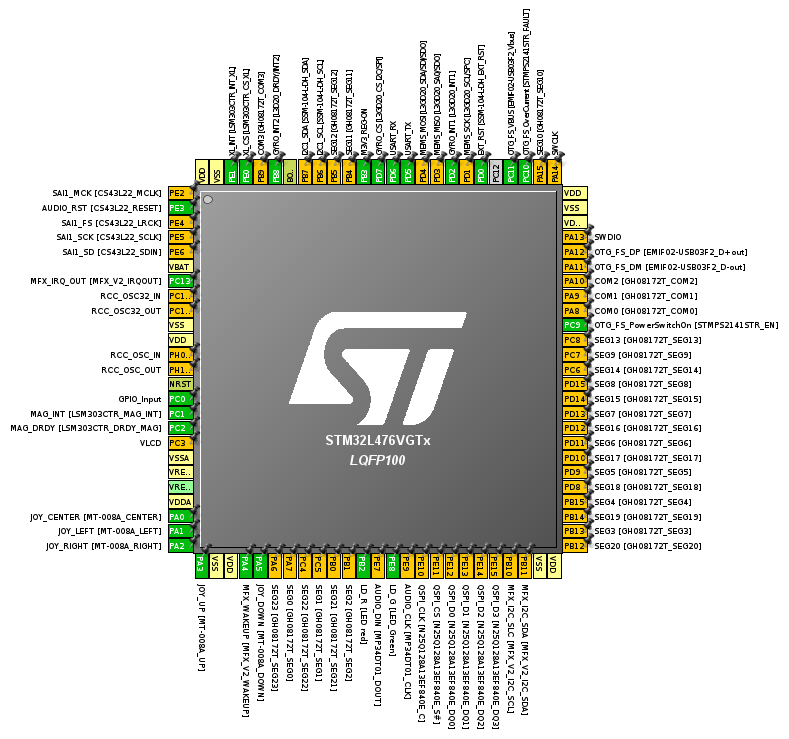
\includegraphics[width=0.85\textwidth]{../img/stm32disco.png}
    \caption{Procesor \textit{STM32L476VG}}
    \label{fig:stm32disco}
\end{figure}

Powyższy procesor może być taktowany zegarem o~częstotliwości równej aż
$80$~[$MHz$], co w~połączeniu z~wbudowanym koprocesorem zmiennoprzecinkowym
powinno pozwolić na symulowanie pracy układu chłodzenia w~czasie rzeczywistym.
W~tym momencie należy również zaznaczyć, iż podobnie jak rdzeń, koprocesor
zmiennoprzecinkowy operuje na słowach 32-bitowych, a~więc w~celu zapewnienia
sprzętowego wykonywania działań na liczbach zmiennoprzecikowych niezbędne było
korzystanie w~trakcie pisania kodu w~języku \textit{C++} z~danych typu
\textit{float}. Teoretycznie zapewniają one mniejszą dokładność, ale w~tym
przypadku pozwalają uniknąć programowego wykonywania operacji oraz zapewniają
dokładność wystarczającą do potrzeb, przez co użycie typu \textit{double} nie
było niezbędne.

Procesor ten przedstawiony został na rysunku~\ref{fig:stm32disco}. Na potrzeby
tego projektu wykorzystywane były jedynie wyprowadzenia PD5 oraz PD6 opisane
jako USART\_TX oraz USART\_RX.

\subsection{Algorytm rozwiązywania równań rożniczkowych}
\indent

Wykorzystana została metoda Rungego--Kutty czwartego rzędu, która jest jedną
z~najpopularniejszych metod numerycznych do iteracyjnego rozwiązywania równań
różniczkowych. Stosowana jest głównie z~powodu prostoty implementacji, dużej
szybkości oraz wysokiego rzędu.
Dysponując równaniem postaci:
\begin{equation*}
    \dot{x} = f\left( t, x \right)
\end{equation*}
w~którym znamy wartość $x(t_0) = x_0$, przyjmujemy dowolną wartość kroku
całkowania $dt$. Iteracyjny wzór metody RK4 jest następujący:
\begin{equation}
    x_{n+1} = x_n + \frac{k_1 + 2 \cdot k_2 + 2 \cdot k_3 + k4}{6}
    \label{equ:rk4}
\end{equation}
gdzie:
\begin{itemize}
    \item $k_1 = dt \cdot f\left( t_n, x_n \right)$,
    \item $k_2 = dt \cdot f\left( t_n + \frac{dt}{2}, x_n + \frac{k_1}{2}
    \right)$,
    \item $k_3 = dt \cdot f\left( t_n + \frac{dt}{2}, x_n + \frac{k_2}{2}
    \right)$,
    \item $k_4 = dt \cdot f\left( t_n + dt, x_n + k_3 \right)$.
\end{itemize}
Powyższy algorytm został zaimplementowany w~języku \textit{C++}.

\newpage
\subsection{Regulatory PID}
\indent

Do wyznaczania sterowań dla pompy wody oraz wentylatorów zostały stworzone
regulatory PID w~wersji dyskretnej opisane równaniem (w~wersji pozycyjnej):
\begin{equation}
    u_n = K_P \cdot e_n + K_I \cdot s_n + K_D \cdot d_n
    \label{equ:reg}
\end{equation}
gdzie:
\begin{itemize}
    \item $u_n$ --~sterowanie,
    \item $K_P$ --~wzmocnienie części proporcjonalnej,
    \item $K_I$ --~wzmocnienie części całkującej,
    \item $K_D$ --~wzmocnienie części różniczkującej,
    \item $e_n$ --~uchyb,
    \item $s_n$ --~suma uchybów dana zależnością:
        \begin{equation}
            s_n = s_{n - 1} + e_n
        \end{equation}
    \item $d_n$ --~różnica uchybów dana zależnością:
        \begin{equation}
            d_n = e_n - e_{n - 1}
        \end{equation}
\end{itemize}

Wartości poszczególnych wzmocnień nie były wyznaczane żadną specjalistyczną
metodą i~najczęściej wykorzystywaną konfiguracją była taka, w~której jedynie
część proporcjonalna posiadała wzmocnienie o~wartości równej $1$. Spowodowane to
było naciskiem na sprawdzenie poprawności samej implementacji modelu oraz
algorytmu rozwiązywania równań różniczkowych, a~także samego panelu
operatorskiego tworzonego na późniejszym etapie prac, aniżeli wyszukiwaniem
optymalnych nastaw względem wybranych wskaźników jakości sterowania.

\subsection{Wyjścia oraz wejścia systemu}
\indent

Stworzony model opisuje układ dwuwejściowy, w~którym możliwe jest sterowanie
pracą pompy wody oraz prędkością obrotową wentylatorów. W~odniesieniu do liczby
wyjść sytuacja jest nieco bardziej złożona, gdyż zależy głównie od wymagań
systemu. Podstawowym wyjściem jest temperatura procesora, która nie może
przekraczać wartości uznanych przez producenta za maksymalne bezpieczne, aby nie
doszło do uszkodzenia struktury krzemowej. Zwykle wynosi ona około
$100$~[$^\circ C$] i~po jej przekroczeniu następuje automatyczne obniżenie
częstotliwości taktowania rdzenia.

W~związku z~tym, w~tworzonym projekcie temperatura ta została wybrana jako
wyjście systemu i~to ona podlegała stabilizacji na zadanym poziomie w~trakcie
pracy układu. Na tej podstawie można stwierdzić, iż obiekt był typu MISO (ang.
Multiple Input Single Output).

W~rzeczywistych układach sytuacja jest bardziej skomplikowana, głównie z~powodu
wytrzymałości elementów systemu chłodzenia. Przykładowa pompa wody
\cite{EKWBpump} powinna pracować dla temperatur wody niższych niż $60$~[$^\circ
C$], w~związku z~czym wielkość ta również powinna podlegać stabilizacji na
poziomie odpowiednio niższym.

Ogromną zaletą rzeczywistych układów, które w~pewnym uproszczeniu zostały
opisane stworzonym modelem, jest jawna postać wszystkich zmiennych stanu, która
możliwa jest do uzyskania poprzez rozmieszczenie odpowiedniej liczby czujników
temperatury w~różnych miejscach pętli chłodzenia. Pozwala to uprościć
sterowanie, gdyż nie ma potrzeby tworzenia obserwatorów stanu, aby estymować
niejawne zmienne.

\subsection{Komunikacja z~komputerem}
\indent

Do komunikacji z~komputerem wykorzystany został port szeregowy. Peryferium
procesora pozwala wykorzystać jego pełną implementację zgodną ze standardem
\textit{RS-232}, lecz w~tym przypadku linie sterujące i~sygnalizujące były
zbędne, w~związku z~czym używano jedynie linii \textit{Rx} oraz \textit{Tx}. Ich
wyprowadzenie na płytce zostało oznaczone czerwonym okręgiem na
rysunku~\ref{fig:discovery}.

\begin{figure}[!ht]
    \centering
    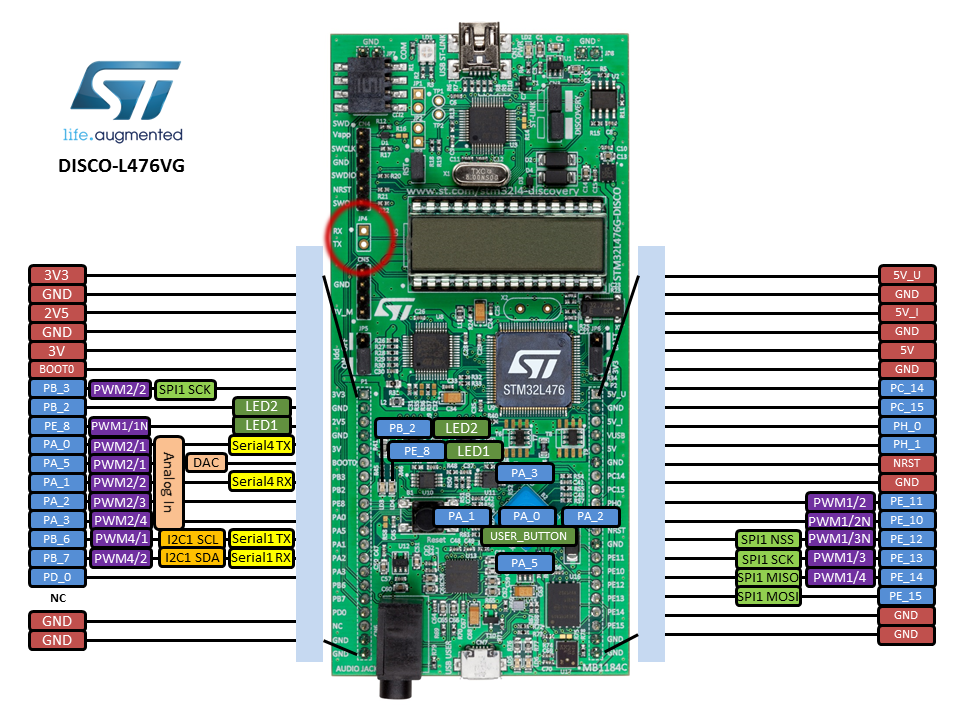
\includegraphics[width=\textwidth]{../img/discovery.png}
    \caption{Oznaczenie linii \textit{Rx} oraz \textit{Tx} na płytce
    \textit{32L476GDISCOVERY}}
    \label{fig:discovery}
\end{figure}

Jak już zostało jednak wspomniane we wcześniejszych rozdziałach, linie te są
jednocześnie podłączone do programatora, który pełni również rolę emulatora
portu szeregowego \textit{RS-232}. Dzięki temu, po podłączeniu płytki do
komputera bardzo szybko można zestawić połączenie z~układem. Podstawowym
zastosowaniem jest tutaj prototypowanie oraz przesyłanie pewnych informacji
kontrolnych, lecz ten projekt, zwłaszcza w~części poświęconej tworzeniu panelu
operatorskiego, miał za zadanie sprawdzić na ile taka komunikacja nadaje się do
zastosowań automatyki. Co ważne, w~początkowych etapach prac, które polegały na
stworzeniu oprogramowania na płytkę, komunikacja przebiegała bez najmniejszych
problemów i~była źródłem wielu informacji pozwalających znaleźć ewentualne
błędy.

Na potrzeby komunikacji przygotowane zostały odpowiednie struktury danych,
identyczne zarówno po stronie mikrokontrolera, jak i~komputera, które
przedstawione zostały na listingu~\ref{lst:commdata}. Dzięki temu, że zarówno
komputer, jak i~mikrokontroler posiadają ten sam system reprezentacji danych
wielobajtowych w~pamięci (LE, ang. Little Endian), nie było potrzeby dokonywania
żadnych pośrednich konwersji w~trakcie wymiany informacji pomiędzy nimi.

\begin{figure}[!ht]
    \lstinputlisting[caption=Struktury
    danych wykorzystywane
    w~komunikacji,label=lst:commdata]{../../dev/WCSim/CommunicationData.h}
\end{figure}
Pierwsza z~nich, \textit{OutData}, zawiera dane dotyczące stanu symulacji
działania układu chłodzenia wysyłane z~mikrokontrolera do komputera:
\begin{itemize}
    \item \textit{mTime} --~aktualny czas działania układu w~sekundach,
    \item \textit{mState} --~tablica zawierająca wszystkie wartości zmiennych
    stanu, zgodnie z~układem równań \eqref{equ:model}.
\end{itemize}

Druga, \textit{PID}, jest strukturą pomocniczą i~zawiera pola z~nastawami
regulatora odpowiadające tym ze wzoru \eqref{equ:reg}:
\begin{itemize}
    \item \textit{mP} --~wartość wzmocnienia części proporcjonalnej,
    \item \textit{mI} --~wartość wzmocnienia części całkującej,
    \item \textit{mD} --~wartość wzmocnienia części różniczkującej.
\end{itemize}

Ostatnia, \textit{InData}, zawiera informacje sterujące przesyłane z~komputera
do mikronkontrolera, które służą do zmiany nastaw regulatorów oraz są
wykorzystywane w~trakcie rozwiązywania układu równań \eqref{equ:model}:
\begin{itemize}
    \item \textit{mPID1} --~nastawy regulatora pompy wody,
    \item \textit{mPID2} --~nastawy regulatora prędkości obrotowej wentylatorów,
    \item \textit{mSetPoint} --~wartość zadana temperatury procesora,
    \item \textit{mPower} --~moc wydzielana w~rdzeniu procesora,
    \item \textit{mTo} --~wartość temperatury otoczenia radiatora.
\end{itemize}
